%2multibyte Version: 5.50.0.2960 CodePage: 65001
% !TeX root = ./Slides_Lez_03_Valori_attesi_condizionati.tex
% ------------------------------------------------------------
% Macro matematiche ufficiali del progetto MQF
% Coerenti con MQF_Notazione.tex
% ------------------------------------------------------------
% Fallback utile per compilazione esterna se qualche titolo resta scritto come \QTR.
% Scientific WorkPlace usa \QTR internamente; in Beamer \QTR{frametitle}{Titolo}
% deve espandersi in \frametitle{Titolo}.

\documentclass[handout]{beamer}%
\usepackage{mathpazo}
%\usepackage{hyperref}
\usepackage{multimedia}
\usepackage{amsmath}
\usepackage{amsfonts}
\usepackage{amssymb}
\usepackage{graphicx}%
\setcounter{MaxMatrixCols}{30}
%TCIDATA{OutputFilter=latex2.dll}
%TCIDATA{Version=5.50.0.2960}
%TCIDATA{Codepage=65001}
%TCIDATA{CSTFile=beamer.cst}
%TCIDATA{Created=Saturday, May 16, 2026 09:09:59}
%TCIDATA{LastRevised=Saturday, May 16, 2026 11:24:58}
%TCIDATA{<META NAME="GraphicsSave" CONTENT="32">}
%TCIDATA{<META NAME="SaveForMode" CONTENT="2">}
%TCIDATA{BibliographyScheme=Manual}
%TCIDATA{<META NAME="DocumentShell" CONTENT="Other Documents\SW\Slides - Beamer">}
%BeginMSIPreambleData
\graphicspath{{../graphics/}}
\providecommand{\U}[1]{\protect\rule{.1in}{.1in}}
%EndMSIPreambleData
\newenvironment{stepenumerate}{\begin{enumerate}[<+->]}{\end{enumerate}}
\newenvironment{stepitemize}{\begin{itemize}[<+->]}{\end{itemize} }
\newenvironment{stepenumeratewithalert}{\begin{enumerate}[<+-| alert@+>]}{\end{enumerate}}
\newenvironment{stepitemizewithalert}{\begin{itemize}[<+-| alert@+>]}{\end{itemize} }
\usetheme{Madrid}
\providecommand{\R}{\mathbb{R}}
\providecommand{\N}{\mathbb{N}}
\providecommand{\E}{\mathbb{E}}
\providecommand{\Prob}{\mathbb{P}}
\providecommand{\Q}{\mathbb{Q}}
\providecommand{\F}{\mathcal{F}}
\providecommand{\B}{\mathcal{B}}
\providecommand{\G}{\mathcal{G}}
\providecommand{\1}{\mathbf{1}}
\providecommand{\Var}{\operatorname{Var}}
\providecommand{\Cov}{\operatorname{Cov}}
\providecommand{\VaR}{\operatorname{VaR}}
\providecommand{\CVaR}{\operatorname{CVaR}}
\providecommand{\argmin}{\operatorname*{arg\,min}}
\providecommand{\argmax}{\operatorname*{arg\,max}}
\providecommand{\EVPI}{\operatorname{EVPI}}
\providecommand{\VSS}{\operatorname{VSS}}
\providecommand{\QTR}[2]{\csname #1\endcsname{#2}}
%BeginMSIPreambleData
\ifx\pdfoutput\relax\let\pdfoutput=\undefined\fi
\newcount\msipdfoutput
\ifx\pdfoutput\undefined\else
\ifcase\pdfoutput\else
\msipdfoutput=1
\ifx\paperwidth\undefined\else
\ifdim\paperheight=0pt\relax\else\pdfpageheight\paperheight\fi
\ifdim\paperwidth=0pt\relax\else\pdfpagewidth\paperwidth\fi
\fi\fi\fi
%EndMSIPreambleData


\title{Lezione 3 - Valori attesi condizionati}
\subtitle{Metodi Quantitativi per la Finanza}
\author[P. Falbo, C. Pelizzari]{{\LARGE Paolo Falbo, Cristian Pelizzari}}
\institute[]{{\large Dipartimento Economia e Management}}
\date[]{}
\titlegraphic{

\includegraphics[width=3.3cm]{../graphics/logo-Unibs-esteso.png}
}

\begin{document}
\maketitle
\section{Apertura}
%****************************************
\subsection{Domanda guida}



%TCIMACRO{\TeXButton{BeginFrame}{\begin{frame}}}%
%BeginExpansion
\begin{frame}%
%EndExpansion

\QTR{frametitle}{Valori attesi condizionati e informazione}

%TCIMACRO{\TeXButton{Transparency}{\setbeamercovered{transparent=20}}}%
%BeginExpansion
\setbeamercovered{transparent=20}%
%EndExpansion

\begin{center}
{\Large Come cambia una media quando cambia l'informazione?}
\end{center}

\medskip

In finanza una valutazione non dipende solo dal payoff futuro, ma anche
dall'informazione disponibile al momento della decisione.

\medskip

\begin{stepitemize}
\item senza informazione aggiuntiva si valuta una media non condizionata;

\item osservando un evento rilevante, la distribuzione dei possibili esiti cambia;

\item osservando una partizione informativa, la valutazione diventa diversa
nei diversi stati osservabili;

\item il valore atteso condizionato formalizza questa revisione:
\[
\E[H\mid\G].
\]
\end{stepitemize}

\medskip

%TCIMACRO{\TeXButton{Transition: Box Out}{\transboxout}}%
%BeginExpansion
\transboxout%
%EndExpansion
%TCIMACRO{\TeXButton{EndFrame}{\end{frame}}}%
%BeginExpansion
\end{frame}%
%EndExpansion

\subsection{Obiettivi della lezione}

%****************************************
%TCIMACRO{\TeXButton{BeginFrame}{\begin{frame}}}%
%BeginExpansion
\begin{frame}%
%EndExpansion

\QTR{frametitle}{Obiettivi della lezione}

%TCIMACRO{\TeXButton{Transparency}{\setbeamercovered{transparent=20}}}%
%BeginExpansion
\setbeamercovered{transparent=20}%
%EndExpansion

Al termine della lezione lo studente deve saper interpretare il valore
atteso condizionato come valutazione coerente con l'informazione disponibile.

\medskip

\begin{stepitemize}
\item richiamare probabilit\`{a} condizionata e distribuzione condizionata;

\item calcolare un valore atteso condizionato rispetto a un evento:
\[
\E[H\mid A];
\]

\item passare da eventi e partizioni a sigma-algebre informative:
\[
\G\subseteq\F;
\]

\item interpretare il valore atteso condizionato come variabile casuale:
\[
\E[H\mid\G];
\]

\item usare le principali regole operative e applicarle a payoff e perdite finanziarie.
\end{stepitemize}

%TCIMACRO{\TeXButton{Transition: Box Out}{\transboxout}}%
%BeginExpansion
\transboxout%
%EndExpansion
%TCIMACRO{\TeXButton{EndFrame}{\end{frame}}}%
%BeginExpansion
\end{frame}%
%EndExpansion
%***********************************

\subsection{Obiettivi della lezione}
%TCIMACRO{\TeXButton{BeginFrame}{\begin{frame}}}%
%BeginExpansion
\begin{frame}%
%EndExpansion

\QTR{frametitle}{Obiettivi della lezione}

%TCIMACRO{\TeXButton{Transparency}{\setbeamercovered{transparent=20}}}%
%BeginExpansion
\setbeamercovered{transparent=20}%
%EndExpansion

Al termine della lezione dovremo saper interpretare il valore atteso
condizionato come valutazione coerente con una data informazione.

\medskip

\begin{stepenumerate}
\item [1.] Richiamare probabilit\`{a} condizionata e distribuzione condizionata
rispetto a un evento osservato.

\item [2.] Definire il valore atteso condizionato rispetto a un evento:
\[
\E[X\mid A].
\]

\item [3.] Passare da eventi singoli a partizioni informative e alla
sigma-algebra generata:
\[
\G=\sigma(B_1,\ldots,B_n).
\]

\item [4.] Interpretare $\E[X\mid\G]$ come variabile casuale osservabile
rispetto all'informazione disponibile.

\item [5.] Usare le principali regole operative e applicarle a payoff,
perdite e scenari di mercato.
\end{stepenumerate}

%TCIMACRO{\TeXButton{Transition: Box Out}{\transboxout}}%
%BeginExpansion
\transboxout%
%EndExpansion
%TCIMACRO{\TeXButton{EndFrame}{\end{frame}}}%
%BeginExpansion
\end{frame}%
%EndExpansion
%*********************************************

%TCIMACRO{\TeXButton{BeginFrame}{\begin{frame}}}%
%BeginExpansion
\begin{frame}%
%EndExpansion

\QTR{frametitle}{Motivazione finanziaria}

%TCIMACRO{\TeXButton{Transparency}{\setbeamercovered{transparent=20}}}%
%BeginExpansion
\setbeamercovered{transparent=20}%
%EndExpansion

Molte grandezze finanziarie sono valutate prima che l'incertezza sia
risolta.

\medskip

\begin{stepitemize}
\item Un \textbf{payoff} futuro $H$ dipende dallo stato di mercato che si
realizzer\`{a}.

\item Una \textbf{perdita} futura $L$ dipende da prezzi, tassi, default e
fattori di rischio non ancora osservati.

\item La valutazione iniziale usa l'informazione disponibile oggi:
\[
\E[H], \qquad \E[L].
\]

\item Se arriva nuova informazione, la valutazione deve essere aggiornata:
\[
\E[H\mid \G], \qquad \E[L\mid \G].
\]
\end{stepitemize}

\medskip

\begin{center}
{\small Condizionare significa valutare una grandezza incerta alla luce
dell'informazione osservabile.}
\end{center}

%TCIMACRO{\TeXButton{Transition: Box Out}{\transboxout}}%
%BeginExpansion
\transboxout%
%EndExpansion
%TCIMACRO{\TeXButton{EndFrame}{\end{frame}}}%
%BeginExpansion
\end{frame}%
%EndExpansion
%*********************************************

\subsection{L'informazione cambia i pesi}
%TCIMACRO{\TeXButton{BeginFrame}{\begin{frame}}}%
%BeginExpansion
\begin{frame}%
%EndExpansion

\QTR{frametitle}{L'informazione cambia i pesi}

%TCIMACRO{\TeXButton{Transparency}{\setbeamercovered{transparent=20}}}%
%BeginExpansion
\setbeamercovered{transparent=20}%
%EndExpansion

Condizionare rispetto ad un evento \textbf{non cambia} il payoff di $H$: cambia l'insieme degli scenari ritenuti compatibili con l'informazione osservata.

\medskip

\begin{stepitemize}
\item Prima dell'informazione, ogni scenario $\omega\in\Omega$ contribuisce
secondo la probabilit\`{a} iniziale $\Prob$.

\item Dopo l'osservazione di un evento $A$, restano rilevanti solo gli
scenari compatibili:
\[
\omega\in A.
\]

\item La media viene ricalcolata usando le \textbf{probabilit\`{a}
condizionate}:
\[
\Prob(H \in,\cdot\,\mid A).
\]

\item Quindi non si modifica la funzione payoff $H$, ma la
\textbf{distribuzione} rispetto alla quale $H$ viene valutato.
\end{stepitemize}


%TCIMACRO{\TeXButton{Transition: Box Out}{\transboxout}}%
%BeginExpansion
\transboxout%
%EndExpansion
%TCIMACRO{\TeXButton{EndFrame}{\end{frame}}}%
%BeginExpansion
\end{frame}%
%EndExpansion
%*********************************************

\subsection{Valore atteso condizionato rispetto a un evento}
%TCIMACRO{\TeXButton{BeginFrame}{\begin{frame}}}%
%BeginExpansion
\begin{frame}%
%EndExpansion

\QTR{frametitle}{Valore atteso condizionato rispetto a un evento}

%TCIMACRO{\TeXButton{Transparency}{\setbeamercovered{transparent=20}}}%
%BeginExpansion
\setbeamercovered{transparent=20}%
%EndExpansion

Sia $H$ una variabile casuale discreta e sia $A\in\F$ un evento con
$\Prob(A)>0$.

\medskip

\begin{stepitemize}
\item Il valore atteso condizionato rispetto ad $A$ \`{e}:
\[
\E[H\mid A]=\sum_h h\,\Prob(H=h\mid A).
\]

\item I pesi della media sono le \textbf{probabilit\`{a} condizionate}:
\[
\Prob(H=h\mid A)
=
\frac{\Prob(\{H=h\}\cap A)}{\Prob(A)}.
\]

\item L'evento $A$ seleziona l'informazione osservata; la media considera
solo gli esiti di $H$ coerenti con tale informazione.

\item $\E[H\mid A]$ \`{e} un numero: rappresenta la valutazione media di
$H$ dopo aver osservato $A$.
\end{stepitemize}

%TCIMACRO{\TeXButton{Transition: Box Out}{\transboxout}}%
%BeginExpansion
\transboxout%
%EndExpansion
%TCIMACRO{\TeXButton{EndFrame}{\end{frame}}}%
%BeginExpansion
\end{frame}%
%EndExpansion
%*********************************************

\subsection{Formula con indicatrice}
%TCIMACRO{\TeXButton{BeginFrame}{\begin{frame}}}%
%BeginExpansion
\begin{frame}%
%EndExpansion

\QTR{frametitle}{Formula con indicatrice}

%TCIMACRO{\TeXButton{Transparency}{\setbeamercovered{transparent=20}}}%
%BeginExpansion
\setbeamercovered{transparent=20}%
%EndExpansion

Sia $A\in\F$ un evento con probabilit\`{a} positiva:
\[
\Prob(A)>0.
\]

\medskip

Il valore atteso condizionato di $X$ dato $A$ pu\`{o} essere scritto come:
\[
\E[X\mid A]
=
\frac{\E[X\mathbf{1}_{A}]}{\Prob(A)}.
\]

\medskip

\begin{stepitemize}
\item $\mathbf{1}_{A}$ seleziona gli scenari in cui l'evento $A$ si verifica.

\item $\E[X\mathbf{1}_{A}]$ somma il contributo di $X$ solo sugli scenari
compatibili con $A$.

\item La divisione per $\Prob(A)$ normalizza la media rispetto alla
probabilit\`{a} dell'evento condizionante.
\end{stepitemize}

\medskip

\begin{center}
{\small La formula mostra che condizionare equivale a restringere e
rinormalizzare la valutazione.}
\end{center}

%TCIMACRO{\TeXButton{Transition: Box Out}{\transboxout}}%
%BeginExpansion
\transboxout%
%EndExpansion
%TCIMACRO{\TeXButton{EndFrame}{\end{frame}}}%
%BeginExpansion
\end{frame}%
%EndExpansion
%*********************************************

\subsection{Caso continuo}
%TCIMACRO{\TeXButton{BeginFrame}{\begin{frame}}}%
%BeginExpansion
\begin{frame}%
%EndExpansion

\QTR{frametitle}{Caso continuo}

%TCIMACRO{\TeXButton{Transparency}{\setbeamercovered{transparent=20}}}%
%BeginExpansion
\setbeamercovered{transparent=20}%
%EndExpansion

Nel caso continuo il condizionamento modifica la \textbf{densit\`{a}}
rispetto alla quale si calcola la media.

\medskip

Se $X$ ha densit\`{a} condizionata $f_{X\mid A}$ dato l'evento $A$, allora:
\[
\E[X\mid A]
=
\int_{\R} x f_{X\mid A}(x)\,dx.
\]

\medskip

\begin{stepitemize}
\item La funzione $f_{X\mid A}$ descrive la distribuzione di $X$ dopo
l'osservazione di $A$.

\item L'integrale \`{e} la stessa operazione di media, ma calcolata con i
\textbf{pesi condizionati}.

\item La grandezza $X$ non viene modificata: cambia la distribuzione
rilevante per la sua valutazione.
\end{stepitemize}

%TCIMACRO{\TeXButton{Transition: Box Out}{\transboxout}}%
%BeginExpansion
\transboxout%
%EndExpansion
%TCIMACRO{\TeXButton{EndFrame}{\end{frame}}}%
%BeginExpansion
\end{frame}%
%EndExpansion

%*************************************

\subsection{Partizioni informative}
%TCIMACRO{\TeXButton{BeginFrame}{\begin{frame}}}%
%BeginExpansion
\begin{frame}%
%EndExpansion

\QTR{frametitle}{Partizioni informative}

%TCIMACRO{\TeXButton{Transparency}{\setbeamercovered{transparent=20}}}%
%BeginExpansion
\setbeamercovered{transparent=20}%
%EndExpansion

Una \textbf{partizione informativa} descrive gli stati che diventano
distinguibili dopo l'osservazione di un segnale.

\medskip

Sia
\[
\Omega = B_1\cup\cdots\cup B_n,
\qquad
B_i\cap B_j=\varnothing \quad \text{se } i\neq j.
\]

\begin{stepitemize}
\item Prima dell'osservazione non sappiamo quale blocco $B_i$ si
realizzer\`{a}.

\item Dopo l'osservazione sappiamo che lo scenario vero appartiene a uno
specifico blocco $B_i$.

\item Per ciascun blocco possiamo calcolare una \textbf{media locale}:
\[
\E[X\mid B_i].
\]

\item La partizione trasforma una sola valutazione globale in una famiglia
di valutazioni condizionate.
\end{stepitemize}

%TCIMACRO{\TeXButton{Transition: Box Out}{\transboxout}}%
%BeginExpansion
\transboxout%
%EndExpansion
%TCIMACRO{\TeXButton{EndFrame}{\end{frame}}}%
%BeginExpansion
\end{frame}%
%EndExpansion
%*********************************************

\subsection{Valore atteso totale}
%TCIMACRO{\TeXButton{BeginFrame}{\begin{frame}}}%
%BeginExpansion
\begin{frame}%
%EndExpansion

\QTR{frametitle}{Valore atteso totale}

%TCIMACRO{\TeXButton{Transparency}{\setbeamercovered{transparent=20}}}%
%BeginExpansion
\setbeamercovered{transparent=20}%
%EndExpansion

La media non condizionata si ottiene ricomponendo le medie locali sui
blocchi della partizione.

\medskip

Se $\{B_1,\ldots,B_n\}$ \`{e} una partizione di $\Omega$ e
$\Prob(B_i)>0$, allora:
\[
\E[X]
=
\sum_{i=1}^{n}\E[X\mid B_i]\Prob(B_i).
\]

\medskip

\begin{stepitemize}
\item $\E[X\mid B_i]$ \`{e} la valutazione di $X$ quando l'informazione
osservata identifica il blocco $B_i$.

\item $\Prob(B_i)$ \`{e} il peso ex ante attribuito a quel possibile stato
informativo.

\item La media globale \`{e} quindi una \textbf{media ponderata} delle
valutazioni condizionate.
\end{stepitemize}

\medskip

\begin{center}
{\small Il valore atteso totale collega la valutazione prima
dell'informazione alle valutazioni dopo l'informazione.}
\end{center}

%TCIMACRO{\TeXButton{Transition: Box Out}{\transboxout}}%
%BeginExpansion
\transboxout%
%EndExpansion
%TCIMACRO{\TeXButton{EndFrame}{\end{frame}}}%
%BeginExpansion
\end{frame}%
%EndExpansion
%*********************************************

\subsection{Figura 3.1: partizione di Omega}
%TCIMACRO{\TeXButton{BeginFrame}{\begin{frame}}}%
%BeginExpansion
\begin{frame}%
%EndExpansion

\QTR{frametitle}{Figura 3.1: partizione di $\Omega$}

%TCIMACRO{\TeXButton{Transparency}{\setbeamercovered{transparent=20}}}%
%BeginExpansion
\setbeamercovered{transparent=20}%
%EndExpansion

\begin{center}
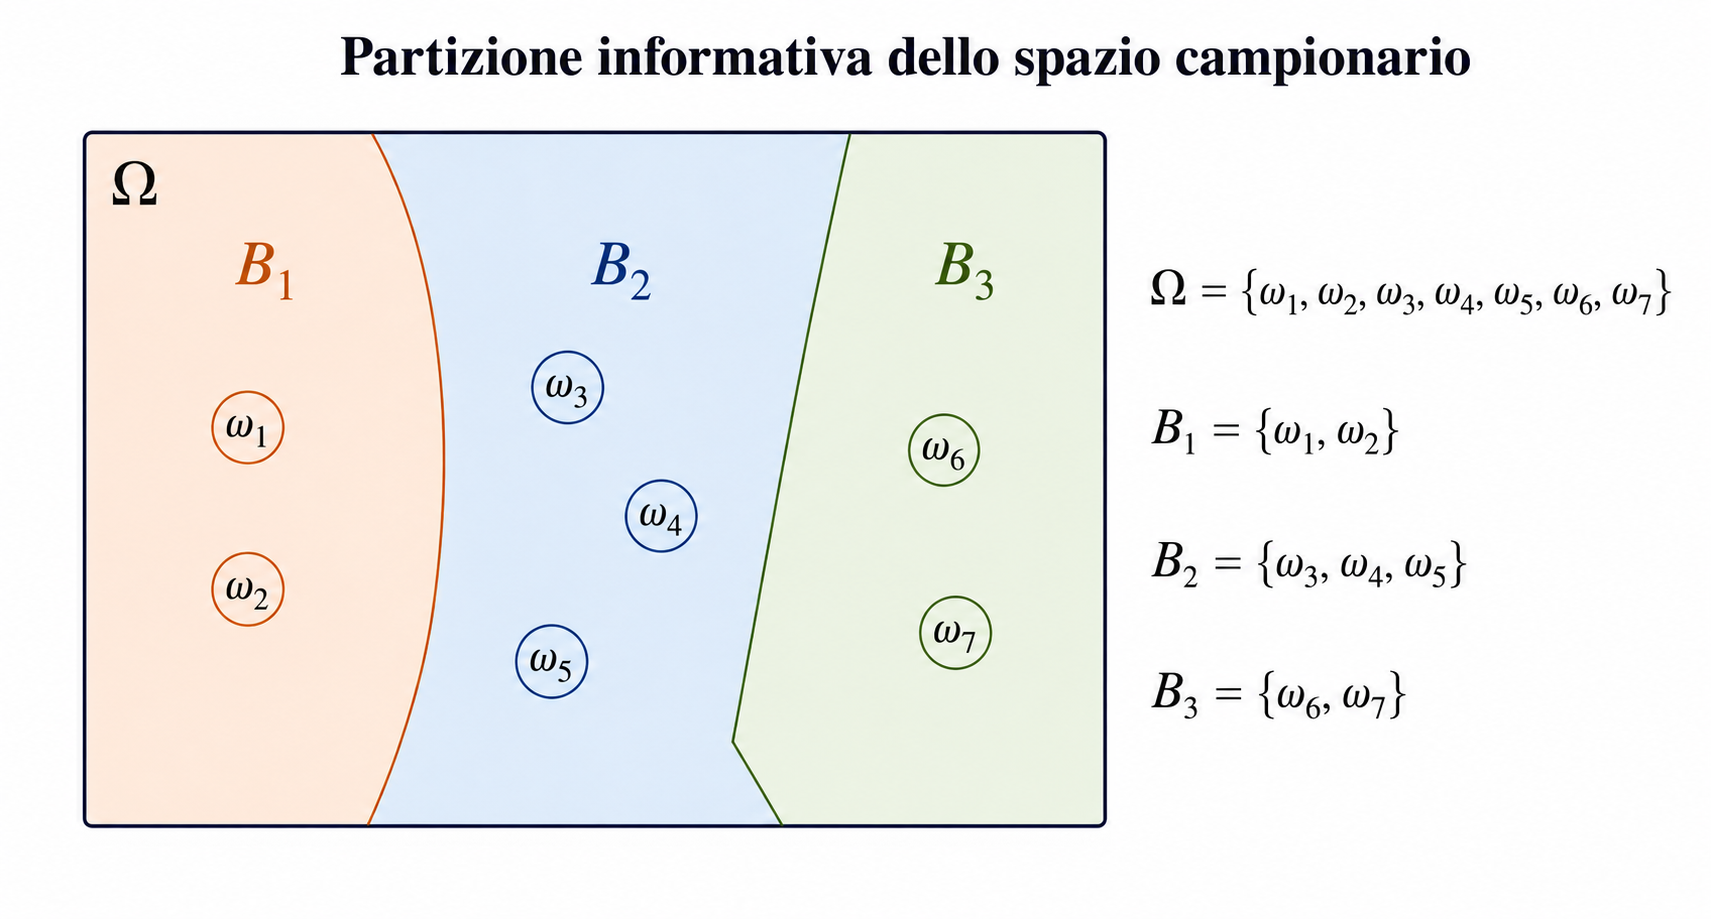
\includegraphics[width=0.72\textwidth]{../graphics/Cap03_Figura_3_1.png}
\end{center}

\begin{stepitemize}
\item Gli eventi elementari rappresentano i singoli scenari $\omega\in\Omega$.

\item Gli eventi $B_1,\ldots,B_n$ raccolgono scenari elementari non distinguibili
dalla stessa \textbf{informazione osservata}.

\item Osservare la partizione significa sapere quale evento $B_i$ si \`{e}
realizzato, senza necessariamente identificare il singolo scenario
elementare $\omega$.
\end{stepitemize}

%TCIMACRO{\TeXButton{Transition: Box Out}{\transboxout}}%
%BeginExpansion
\transboxout%
%EndExpansion
%TCIMACRO{\TeXButton{EndFrame}{\end{frame}}}%
%BeginExpansion
\end{frame}%
%EndExpansion
%*********************************************

\subsection{Sigma-algebra generata e atomi}
%TCIMACRO{\TeXButton{BeginFrame}{\begin{frame}}}%
%BeginExpansion
\begin{frame}%
%EndExpansion

\QTR{frametitle}{Sigma-algebra generata e atomi}

%TCIMACRO{\TeXButton{Transparency}{\setbeamercovered{transparent=20}}}%
%BeginExpansion
\setbeamercovered{transparent=20}%
%EndExpansion

Data una partizione $\{B_1,\ldots,B_n\}$ di $\Omega$, l'informazione
osservabile \`{e} descritta dalla sigma-algebra
\[
\G=\sigma(B_1,\ldots,B_n).
\]

\medskip

\begin{stepitemize}
\item Gli \textbf{atomi} di $\G$ sono gli eventi della partizione:
\[
B_1,\ldots,B_n.
\]

\item Gli \textbf{eventi osservabili} sono le unioni di atomi:
\[
B_{i_1}\cup\cdots\cup B_{i_k}.
\]

\item Un evento \`{e} osservabile rispetto a $\G$ se pu\`{o} essere
deciso conoscendo quale evento $B_i$ si \`{e} realizzato.

\item La sigma-algebra $\G$ formalizza quindi il contenuto informativo
della partizione.
\end{stepitemize}

%TCIMACRO{\TeXButton{Transition: Box Out}{\transboxout}}%
%BeginExpansion
\transboxout%
%EndExpansion
%TCIMACRO{\TeXButton{EndFrame}{\end{frame}}}%
%BeginExpansion
\end{frame}%
%EndExpansion
%*********************************************

\subsection{\texorpdfstring{$\E[X\mid\G]$ come variabile casuale}{E[X|G] come variabile casuale}}
%TCIMACRO{\TeXButton{BeginFrame}{\begin{frame}}}%
%BeginExpansion
\begin{frame}%
%EndExpansion

\QTR{frametitle}{\texorpdfstring{$\E[X\mid\G]$ come variabile casuale}{E[X|G] come variabile casuale}}

%TCIMACRO{\TeXButton{Transparency}{\setbeamercovered{transparent=20}}}%
%BeginExpansion
\setbeamercovered{transparent=20}%
%EndExpansion

Se $\G=\sigma(B_1,\ldots,B_n)$, il valore atteso condizionato rispetto a
$\G$ \`{e} la variabile casuale
\[
\E[X\mid\G]
=
\sum_{i=1}^{n}\E[X\mid B_i]\mathbf{1}_{B_i}.
\]

\medskip

\begin{stepitemize}
\item Su ciascun atomo $B_i$, la variabile $\E[X\mid\G]$ \`{e}
\textbf{costante}.

\item Il valore assunto su $B_i$ \`{e} la media condizionata
$\E[X\mid B_i]$.

\item Condizionare rispetto a un \textbf{evento} $A$ produce un numero:
\[
\E[X\mid A].
\]

\item Condizionare rispetto a una \textbf{sigma-algebra} $\G$ produce una
variabile casuale osservabile rispetto a $\G$.
\end{stepitemize}

%TCIMACRO{\TeXButton{Transition: Box Out}{\transboxout}}%
%BeginExpansion
\transboxout%
%EndExpansion
%TCIMACRO{\TeXButton{EndFrame}{\end{frame}}}%
%BeginExpansion
\end{frame}%
%EndExpansion

%*********************************************

\subsection{Esempio con sette eventi elementari}
%TCIMACRO{\TeXButton{BeginFrame}{\begin{frame}}}%
%BeginExpansion
\begin{frame}%
%EndExpansion

\QTR{frametitle}{Esempio con sette eventi elementari}

%TCIMACRO{\TeXButton{Transparency}{\setbeamercovered{transparent=20}}}%
%BeginExpansion
\setbeamercovered{transparent=20}%
%EndExpansion

Sia $\Omega=\{\omega_1,\ldots,\omega_7\}$ e sia
$\G=\sigma(B_1,B_2,B_3)$, con
\[
B_1=\{\omega_1,\omega_2\},\quad
B_2=\{\omega_3,\omega_4,\omega_5\},\quad
B_3=\{\omega_6,\omega_7\}.
\]

\medskip

\begin{center}
{\scriptsize
\begin{tabular}{c|c|c|c}
Evento della partizione & Probabilit\`{a} & Valori di $H$ &
Media condizionata \\ \hline
$B_1$ & $0.10,\ 0.15$ & $130,\ 110$ &
$\E[H\mid B_1]=118$ \\
$B_2$ & $0.15,\ 0.20,\ 0.10$ & $100,\ 90,\ 80$ &
$\E[H\mid B_2]=91.111$ \\
$B_3$ & $0.18,\ 0.12$ & $70,\ 50$ &
$\E[H\mid B_3]=62$
\end{tabular}
}
\end{center}

\medskip

La variabile casuale condizionata \`{e} quindi:
\[
\E[H\mid\G]
=
118\,\mathbf{1}_{B_1}
+
91.111\,\mathbf{1}_{B_2}
+
62\,\mathbf{1}_{B_3}.
\]

\medskip

\begin{center}
{\small $\E[H\mid\G]$ assegna a ogni scenario la previsione media del
relativo \textbf{evento informativo}.}
\end{center}

%TCIMACRO{\TeXButton{Transition: Box Out}{\transboxout}}%
%BeginExpansion
\transboxout%
%EndExpansion
%TCIMACRO{\TeXButton{EndFrame}{\end{frame}}}%
%BeginExpansion
\end{frame}%
%EndExpansion
%*********************************************

\subsection{Figura 3.3: payoff e previsione condizionata}
%TCIMACRO{\TeXButton{BeginFrame}{\begin{frame}}}%
%BeginExpansion
\begin{frame}%
%EndExpansion

\QTR{frametitle}{Figura 3.3: payoff e previsione condizionata}

%TCIMACRO{\TeXButton{Transparency}{\setbeamercovered{transparent=20}}}%
%BeginExpansion
\setbeamercovered{transparent=20}%
%EndExpansion

\begin{center}
%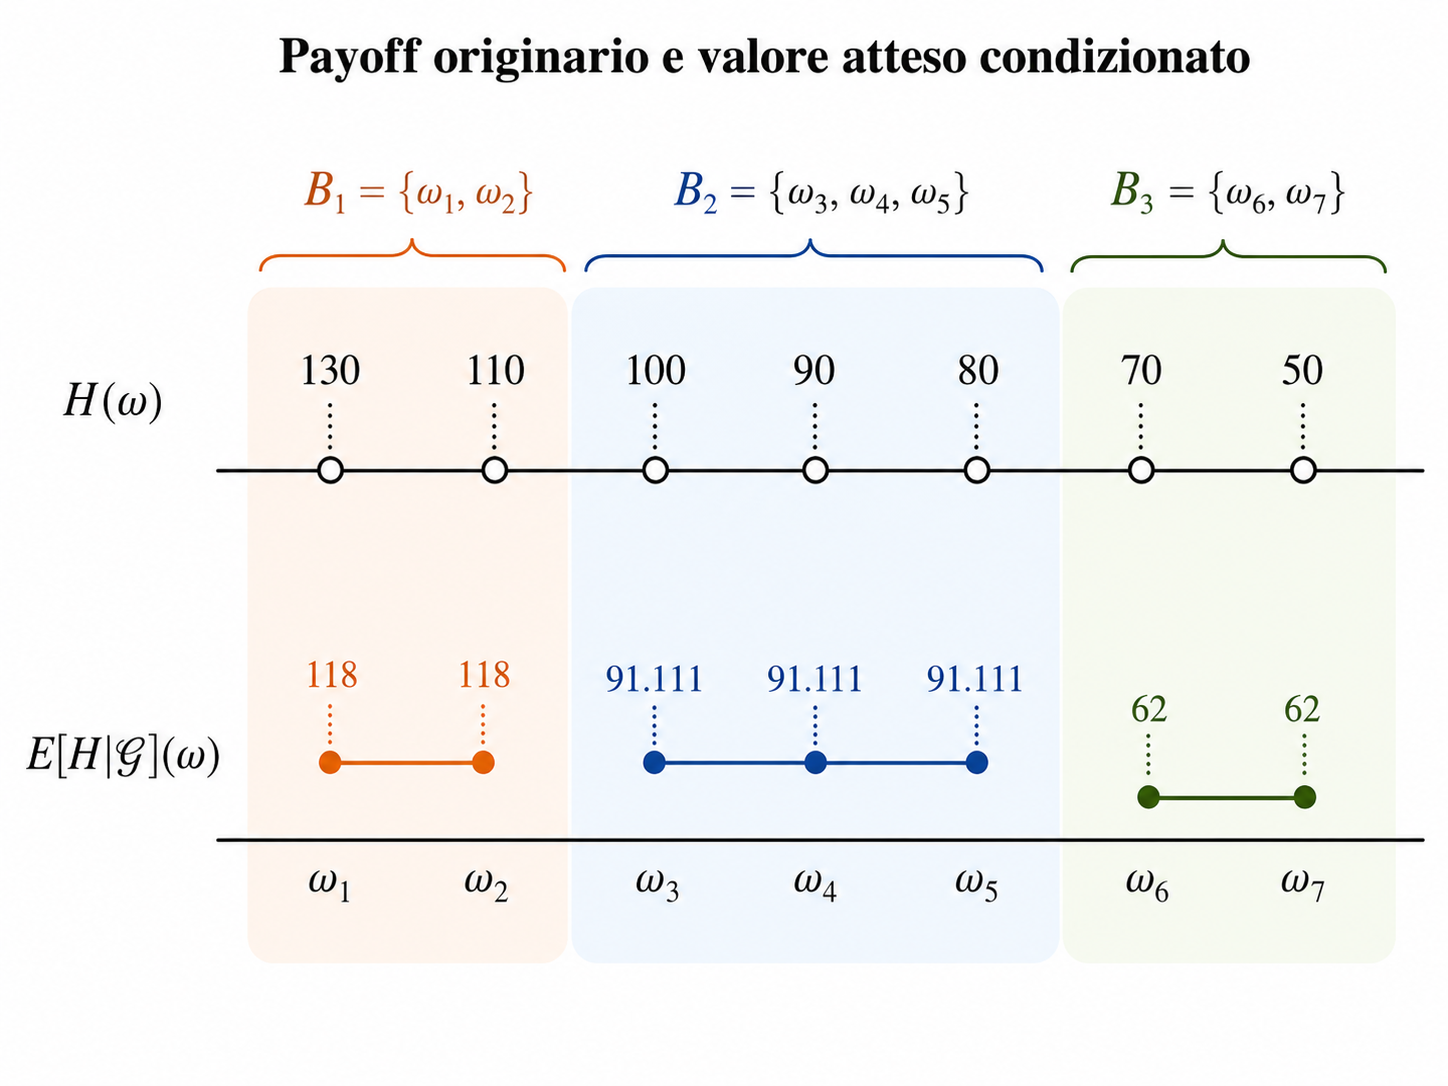
\includegraphics[width=0.72\textwidth]{Cap03_Figura_3_3.png}
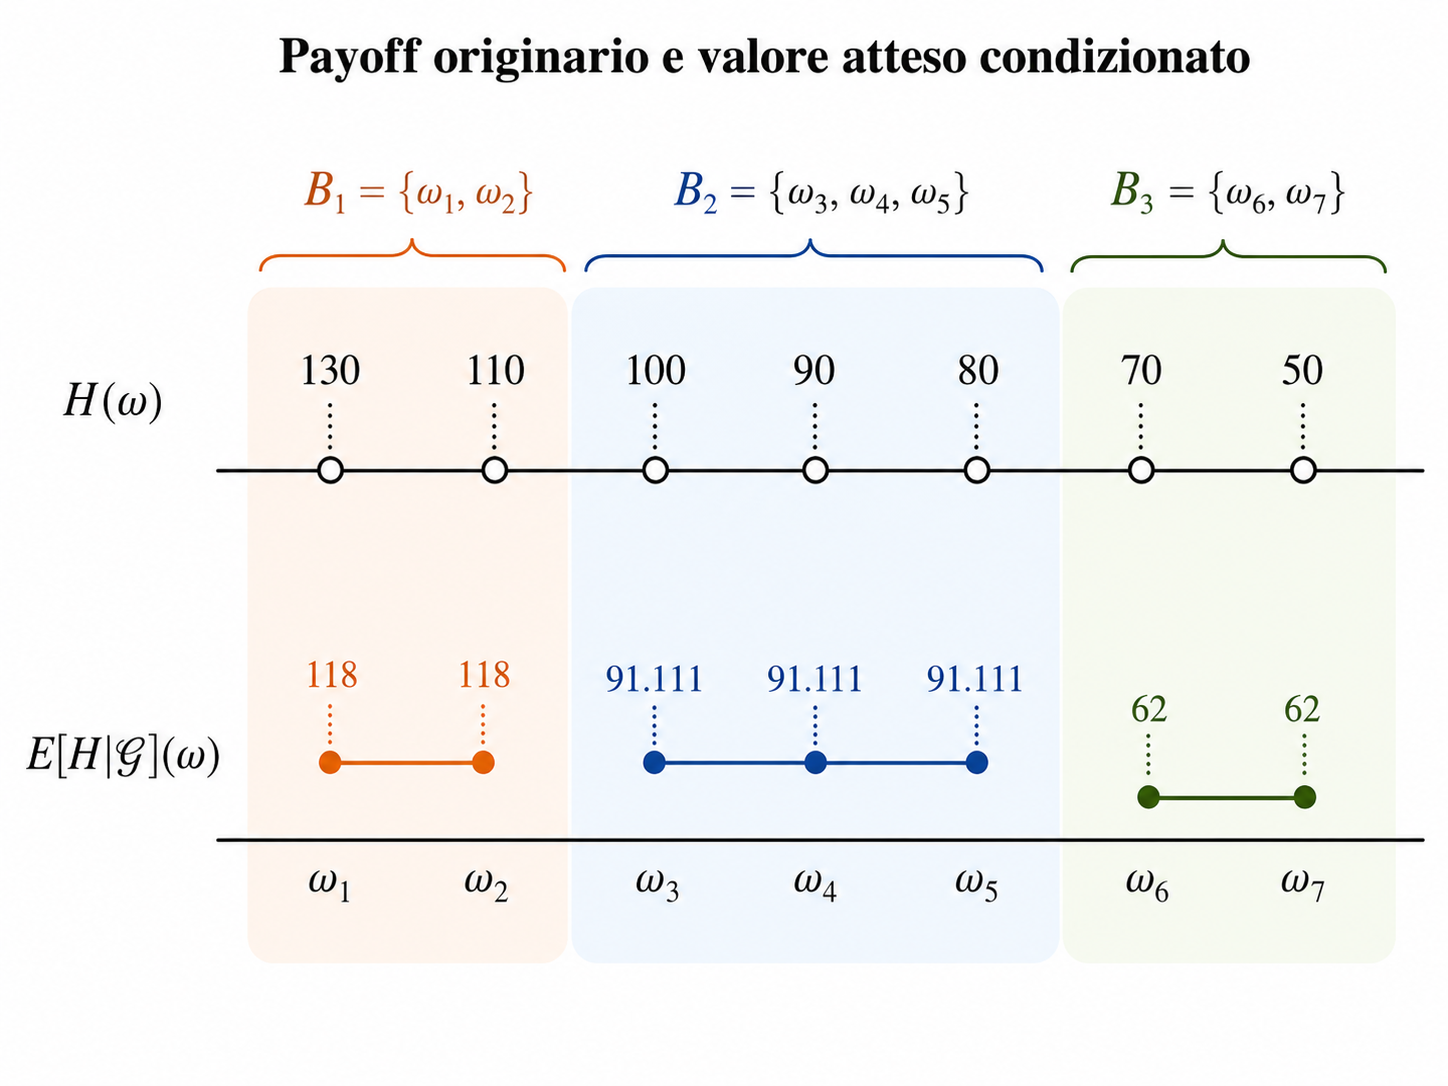
\includegraphics[width=0.76\textwidth,trim=0 60 0 10,clip]{Cap03_Figura_3_3.png}
\end{center}

\vspace{-4mm}

\begin{stepitemize}
\item Il payoff $H$ distingue i sette eventi elementari
$\omega_1,\ldots,\omega_7$.

\item La previsione condizionata $\E[H\mid\G]$ \`{e} invece
\textbf{costante} su ciascun atomo di $\G$.

\end{stepitemize}

%TCIMACRO{\TeXButton{Transition: Box Out}{\transboxout}}%
%BeginExpansion
\transboxout%
%EndExpansion
%TCIMACRO{\TeXButton{EndFrame}{\end{frame}}}%
%BeginExpansion
\end{frame}%
%EndExpansion

%*********************************************

\subsection{Evento osservabile non atomico}
%TCIMACRO{\TeXButton{BeginFrame}{\begin{frame}}}%
%BeginExpansion
\begin{frame}%
%EndExpansion

\QTR{frametitle}{Evento osservabile non atomico}

%TCIMACRO{\TeXButton{Transparency}{\setbeamercovered{transparent=20}}}%
%BeginExpansion
\setbeamercovered{transparent=20}%
%EndExpansion

Sia $\G=\sigma(B_1,B_2,B_3)$ e consideriamo l'evento osservabile
\[
A=B_1\cup B_2.
\]

\medskip

Allora:
\[
\Prob(A)=0.25+0.45=0.70,
\]
\[
\E[H\mid A]
=
\frac{118\cdot 0.25+91.111\cdot 0.45}{0.70}
\simeq
100.714.
\]

\medskip

\begin{stepitemize}
\item $A$ \`{e} un \textbf{evento osservabile}, ma non un atomo di $\G$.

\item $\E[H\mid A]$ \`{e} una media unica sull'unione $B_1\cup B_2$.

\item $\E[H\mid\G]$ mantiene invece separate le previsioni sugli atomi:
\[
118 \ \text{su } B_1,
\qquad
91.111 \ \text{su } B_2,
\qquad
62 \ \text{su } B_3.
\]
\end{stepitemize}

%TCIMACRO{\TeXButton{Transition: Box Out}{\transboxout}}%
%BeginExpansion
\transboxout%
%EndExpansion
%TCIMACRO{\TeXButton{EndFrame}{\end{frame}}}%
%BeginExpansion
\end{frame}%
%EndExpansion
%*********************************************

\subsection{Figura 3.4: informazione fine e grossolana}
%TCIMACRO{\TeXButton{BeginFrame}{\begin{frame}}}%
%BeginExpansion
\begin{frame}%
%EndExpansion

\QTR{frametitle}{Figura 3.4: informazione fine e grossolana}

%TCIMACRO{\TeXButton{Transparency}{\setbeamercovered{transparent=20}}}%
%BeginExpansion
\setbeamercovered{transparent=20}%
%EndExpansion

{\centering
%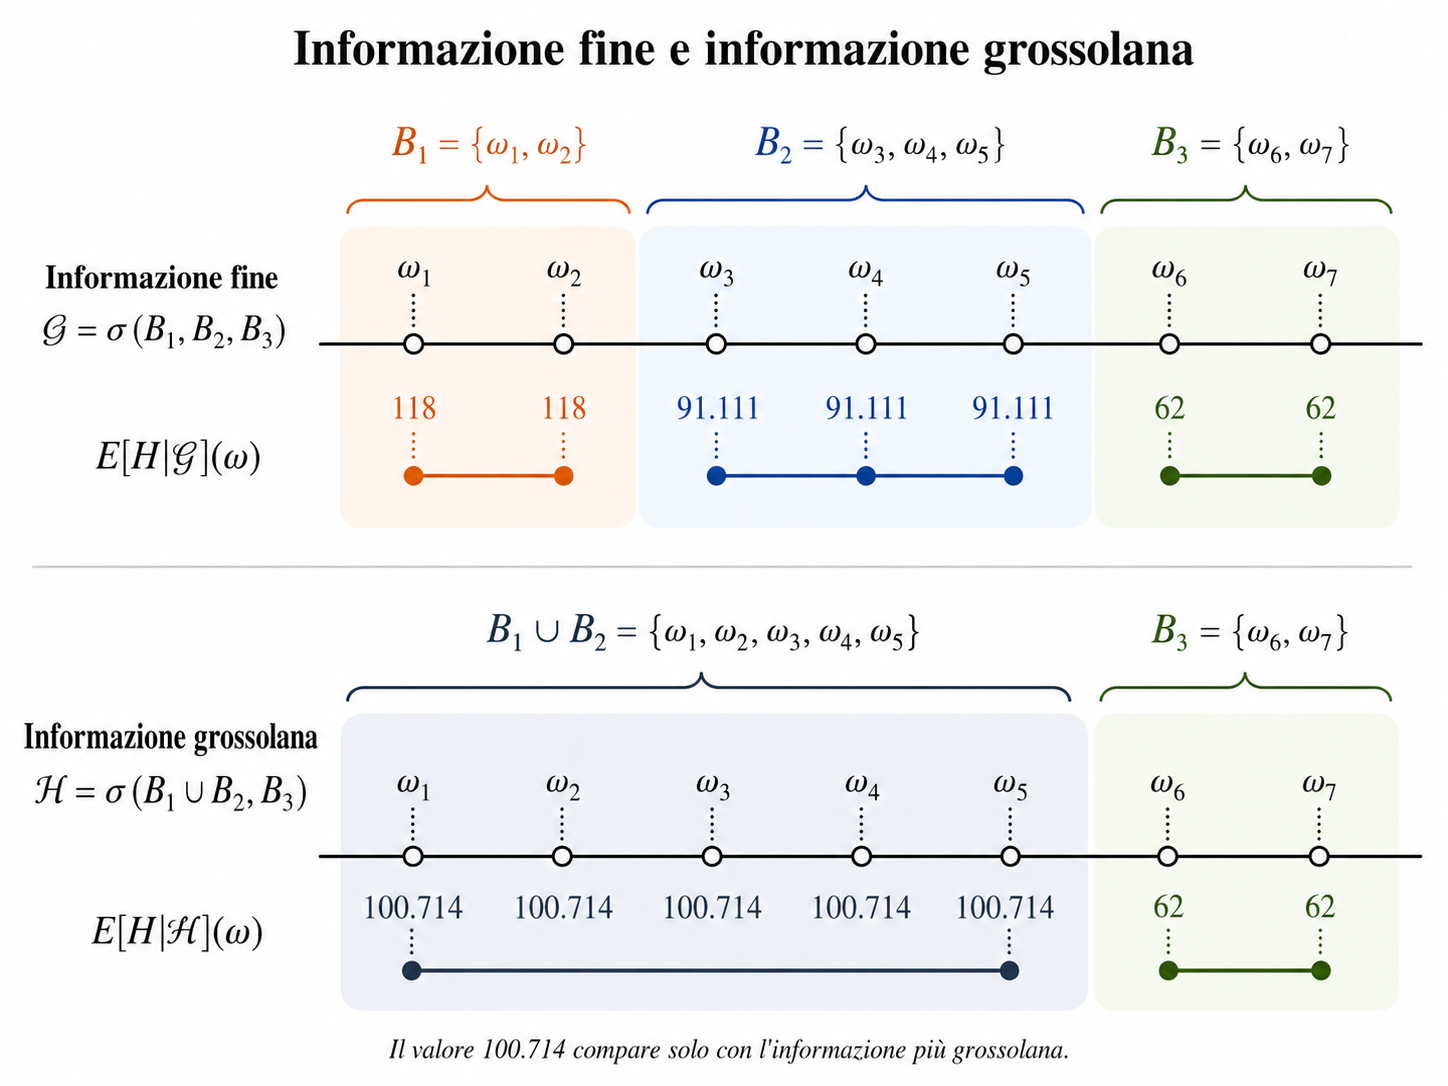
\includegraphics[width=0.74\textwidth]{Cap03_Figura_3_4.png}
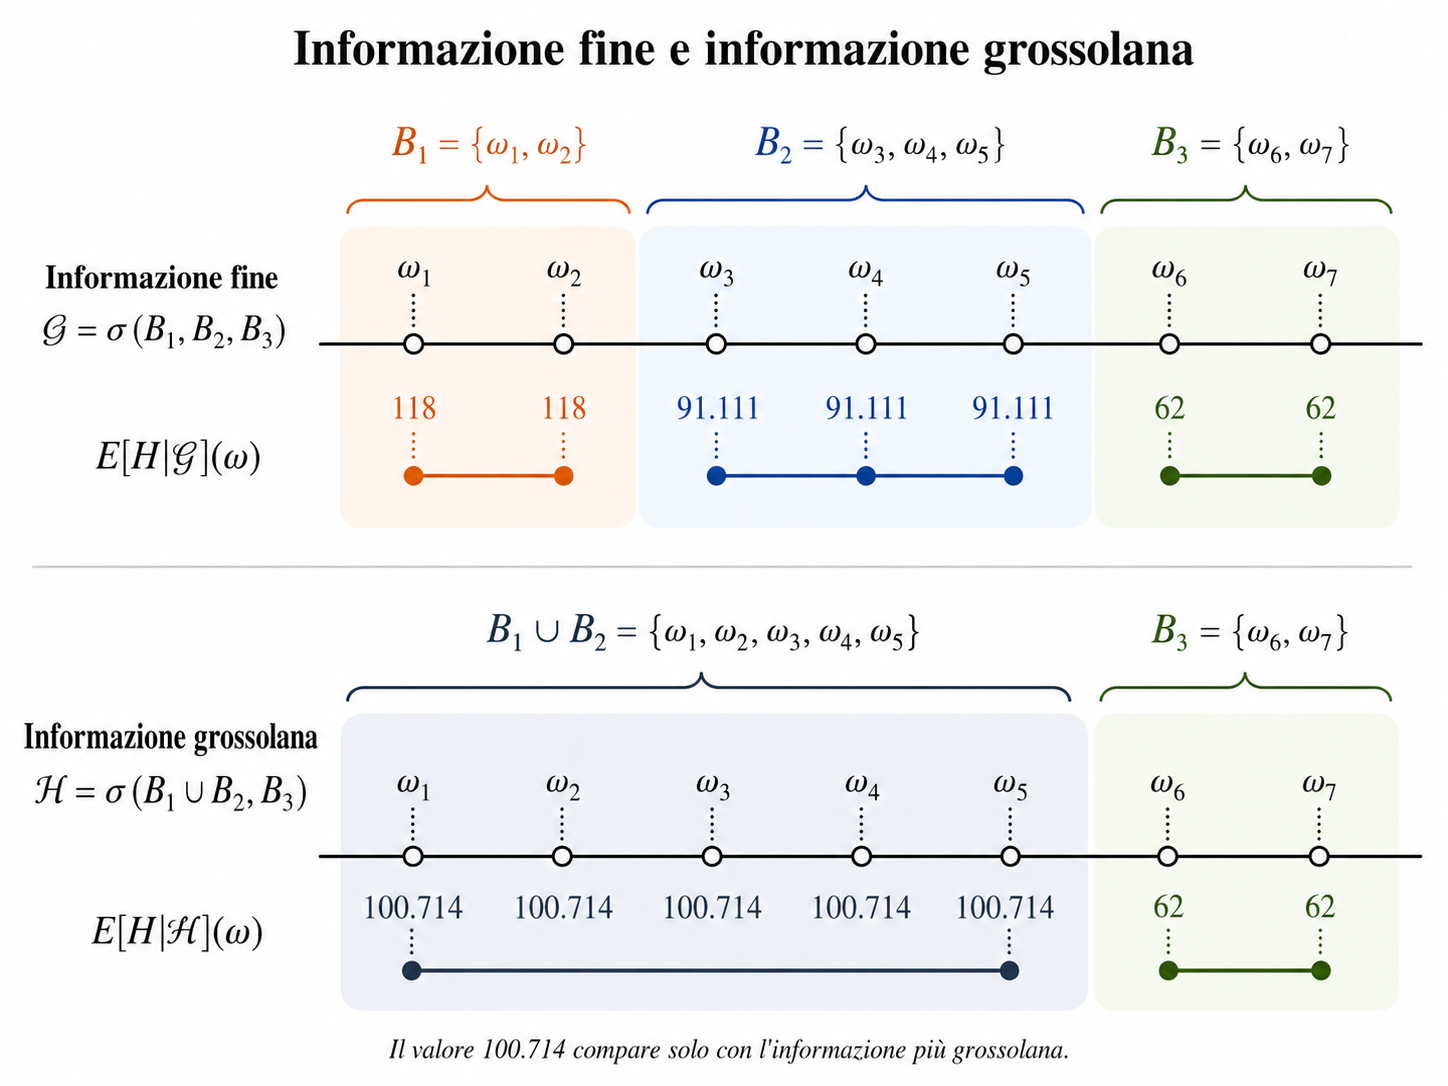
\includegraphics[
  width=0.70\textwidth,
  trim=0 50 0 110,
  clip
]{Cap03_Figura_3_4.png}
\par}

\vspace{-4mm}

\begin{stepitemize}
\item La sigma-algebra $\G$ rappresenta un'informazione pi\`{u}
\textbf{fine}: distingue un numero maggiore di eventi.

\item La sigma-algebra $\mathcal{H}$ rappresenta un'informazione pi\`{u}
\textbf{grossolana}: aggrega alcuni eventi distinguibili da $\G$.

\item Se $\mathcal{H}\subseteq\G$, ogni evento osservabile con
$\mathcal{H}$ \`{e} osservabile anche con $\G$, ma non viceversa.

\end{stepitemize}

%TCIMACRO{\TeXButton{Transition: Box Out}{\transboxout}}%
%BeginExpansion
\transboxout%
%EndExpansion
%TCIMACRO{\TeXButton{EndFrame}{\end{frame}}}%
%BeginExpansion
\end{frame}%
%EndExpansion
%*********************************************

\subsection{Regole operative: mappa generale}
%TCIMACRO{\TeXButton{BeginFrame}{\begin{frame}}}%
%BeginExpansion
\begin{frame}%
%EndExpansion

\QTR{frametitle}{Regole operative: mappa generale}

%TCIMACRO{\TeXButton{Transparency}{\setbeamercovered{transparent=20}}}%
%BeginExpansion
\setbeamercovered{transparent=20}%
%EndExpansion

Per variabili integrabili, il valore atteso condizionato soddisfa alcune
\textbf{regole operative} fondamentali.

\medskip

{\small
\begin{stepenumerate}
\item [1.] \textbf{Linearit\`{a}}:
$\E[aX+bY\mid\G]=a\E[X\mid\G]+b\E[Y\mid\G]$.

\item [2.] \textbf{Estrazione di ci\`{o} che \`{e} noto}: se $Z$ \`{e}
$\G$-misurabile, allora
$\E[ZX\mid\G]=Z\E[X\mid\G]$.

\item [3.] \textbf{Torre}: se $\mathcal{H}\subseteq\G$, allora
$\E[\E[X\mid\G]\mid\mathcal{H}]=\E[X\mid\mathcal{H}]$.

\item [4.] \textbf{Indipendenza da $\G$}: se $X$ \`{e} indipendente da
$\G$, allora $\E[X\mid\G]=\E[X]$.

\item [5.] \textbf{Indipendenza fra variabili casuali}: se $X$ e $Z$ sono
indipendenti, allora $\E[X\mid Z]=\E[X]$, dove
$\E[X\mid Z]=\E[X\mid\sigma(Z)]$.

\item [6.] \textbf{Jensen condizionata}: se $\varphi$ \`{e} convessa,
$\varphi(\E[X\mid\G])\leq \E[\varphi(X)\mid\G]$.
\end{stepenumerate}
}

%TCIMACRO{\TeXButton{Transition: Box Out}{\transboxout}}%
%BeginExpansion
\transboxout%
%EndExpansion
%TCIMACRO{\TeXButton{EndFrame}{\end{frame}}}%
%BeginExpansion
\end{frame}%
%EndExpansion

%*********************************************

\subsection{Torre: due livelli informativi}
%TCIMACRO{\TeXButton{BeginFrame}{\begin{frame}}}%
%BeginExpansion
\begin{frame}%
%EndExpansion

\QTR{frametitle}{Torre: due livelli informativi}

%TCIMACRO{\TeXButton{Transparency}{\setbeamercovered{transparent=20}}}%
%BeginExpansion
\setbeamercovered{transparent=20}%
%EndExpansion

Consideriamo un payoff terminale $X$ e due segnali osservabili sullo
stato del mercato.

\medskip

\[
\mathcal{G}_1
=
\sigma(N,S),
\]
dove:
\[
N=\{\text{mercato normale}\},
\qquad
S=\{\text{mercato stressato}\}.
\]

\medskip

Supponiamo poi che l'informazione pi\`{u} fine distingua, dentro ciascuno
stato, anche la classe di spread:
\[
\mathcal{G}_2
=
\sigma(N_L,N_H,S_L,S_H).
\]

\medskip

Gli eventi di $\mathcal{G}_1$ sono unioni di eventi di $\mathcal{G}_2$:
\[
N=N_L\cup N_H,
\qquad
S=S_L\cup S_H.
\]

\medskip

Quindi:
\[
\mathcal{G}_1\subseteq\mathcal{G}_2.
\]

%TCIMACRO{\TeXButton{Transition: Box Out}{\transboxout}}%
%BeginExpansion
\transboxout%
%EndExpansion
%TCIMACRO{\TeXButton{EndFrame}{\end{frame}}}%
%BeginExpansion
\end{frame}%
%EndExpansion
%*********************************************

\section{Migliore previsione}

\subsection{Criterio dell'errore quadratico medio}
 
%TCIMACRO{\TeXButton{BeginFrame}{\begin{frame}}}%
%BeginExpansion
\begin{frame}%
%EndExpansion
 
\QTR{frametitle}{\texorpdfstring{$\E[X\mid\G]$ come migliore previsione: il criterio}{E[X|G] come migliore previsione: il criterio}}
 
%TCIMACRO{\TeXButton{Transparency}{\setbeamercovered{transparent=20}}}%
%BeginExpansion
\setbeamercovered{transparent=20}%
%EndExpansion
 
\textbf{Problema.} Data l'informazione $\G$, quale variabile casuale
$\G$-misurabile approssima meglio $X$?
 
\medskip
 
\textbf{Criterio.} Minimizzare l'errore quadratico medio tra tutte
le previsioni ammissibili $Y$:
\[
\min_{Y} \; \E\left[(X - Y)^2\right].
\]
 
\medskip
 
\begin{stepitemize}
 
\item Una previsione $Y$ \`{e} \textbf{ammissibile} se \`{e}
$\G$-misurabile: non pu\`{o} usare informazione che $\G$ non contiene.
 
\item L'errore quadratico medio misura quanto $Y$ si discosta da $X$
in media, su tutti gli scenari.
 
\item Il criterio seleziona la previsione che minimizza tale scarto,
rispettando il vincolo informativo.
 
\end{stepitemize}
 
%TCIMACRO{\TeXButton{Transition: Box Out}{\transboxout}}%
%BeginExpansion
\transboxout
%EndExpansion%
%TCIMACRO{\TeXButton{EndFrame}{\end{frame}}}%
%BeginExpansion
\end{frame}%
%EndExpansion
% **************************
 
\subsection{La soluzione}
 
%TCIMACRO{\TeXButton{BeginFrame}{\begin{frame}}}%
%BeginExpansion
\begin{frame}%
%EndExpansion
 
\QTR{frametitle}{$\E[X\mid\G]$ come migliore previsione: la soluzione}
 
%TCIMACRO{\TeXButton{Transparency}{\setbeamercovered{transparent=20}}}%
%BeginExpansion
\setbeamercovered{transparent=20}%
%EndExpansion
 
Se $\G = \sigma(B_1,\ldots,B_n)$, ogni previsione ammissibile deve
essere costante su ciascun atomo $B_i$:
\[
Y = \sum_{i=1}^{n} y_i \1_{B_i}.
\]
 
\begin{stepitemize}
 
\item La scelta di $y_i$ \`{e} libera, ma vincolata: tutti gli scenari
in $B_i$ devono ricevere lo stesso valore previsto.
 
\item La scelta ottima \`{e} la media di $X$ sull'atomo $B_i$:
\[
y_i = \E[X \mid B_i].
\]
 
\item La previsione ottima coincide quindi con il valore atteso
condizionato rispetto a $\G$:
\[
Y^* = \E[X \mid \G] = \sum_{i=1}^{n} \E[X \mid B_i] \1_{B_i}.
\]
 
\end{stepitemize}
 
\begin{center}
{\small $\E[X\mid\G]$ \`{e} l'unica previsione che usa tutta
l'informazione di $\G$ e niente di pi\`{u}.}
\end{center}
 
%TCIMACRO{\TeXButton{Transition: Box Out}{\transboxout}}%
%BeginExpansion
\transboxout
%EndExpansion%
%TCIMACRO{\TeXButton{EndFrame}{\end{frame}}}%
%BeginExpansion
\end{frame}%
%EndExpansion
% **************************
 
\subsection{Verifica sull'esempio}
 
%TCIMACRO{\TeXButton{BeginFrame}{\begin{frame}}}%
%BeginExpansion
\begin{frame}%
%EndExpansion
 
\QTR{frametitle}{Verifica sull'esempio a 7 scenari}
 
%TCIMACRO{\TeXButton{Transparency}{\setbeamercovered{transparent=20}}}%
%BeginExpansion
\setbeamercovered{transparent=20}%
%EndExpansion
 
Riprendiamo la partizione $\G = \sigma(B_1, B_2, B_3)$ e il payoff $H$.
 
\medskip
 
Qualsiasi previsione basata su $\G$ deve avere la forma:
\[
Y = y_1 \1_{B_1} + y_2 \1_{B_2} + y_3 \1_{B_3}.
\]
 
\begin{stepitemize}
 
\item Perch\'{e} $y_1 = 118$? Su $B_1 = \{\omega_1, \omega_2\}$,
con $H(\omega_1) = 130$ e $H(\omega_2) = 110$, qualsiasi altra
costante aumenta l'errore quadratico medio.
 
\item Analogamente: $y_2 = 91.1$ su $B_2$
e $y_3 = 62$ su $B_3$.
 
\item La previsione ottima \`{e}:
\[
\E[H\mid\G] = 118\,\1_{B_1} + 91.1\,\1_{B_2} + 62\,\1_{B_3}.
\]
 
\end{stepitemize}
 
\medskip
 
\textbf{Interpretazione.} $\G$ non distingue $\omega_1$ da $\omega_2$:
la migliore previsione compatibile con $\G$ assegna a entrambi
la media interna all'atomo.
 
%TCIMACRO{\TeXButton{Transition: Box Out}{\transboxout}}%
%BeginExpansion
\transboxout
%EndExpansion%
%TCIMACRO{\TeXButton{EndFrame}{\end{frame}}}%
%BeginExpansion
\end{frame}%
%EndExpansion
% **************************

\subsection{Il portafoglio e la perdita}
 
%TCIMACRO{\TeXButton{BeginFrame}{\begin{frame}}}%
%BeginExpansion
\begin{frame}%
%EndExpansion
 
\QTR{frametitle}{Il portafoglio e la perdita $L$}
 
%TCIMACRO{\TeXButton{Transparency}{\setbeamercovered{transparent=20}}}%
%BeginExpansion
\setbeamercovered{transparent=20}%
%EndExpansion
 
Un portafoglio pu\`{o} trovarsi in sette stati di mercato. La perdita $L$ (in milioni di euro) \`{e}:
 
\medskip
 
\begin{center}
\begin{tabular}{c|l|c|c}
$\omega$ & Stato & $\Prob(\omega)$ & $L(\omega)$ \\
\hline
$\omega_1$ & espansione forte    & 0.10 & 2  \\
$\omega_2$ & espansione moderata & 0.15 & 4  \\
$\omega_3$ & crescita stabile    & 0.15 & 6  \\
$\omega_4$ & stagnazione         & 0.20 & 8  \\
$\omega_5$ & rallentamento       & 0.10 & 12 \\
$\omega_6$ & recessione moderata & 0.18 & 20 \\
$\omega_7$ & recessione severa   & 0.12 & 35 \\
\end{tabular}
\end{center}
 
\medskip
 
La perdita media ex ante \`{e}:
\[
\E[L] = 0.10\cdot2 + 0.15\cdot4 + \cdots + 0.12\cdot35 = 12.30.
\]
 
\medskip
 
\textbf{Domanda.} Come cambia la previsione della perdita quando arriva informazione sullo stato di mercato?
 
%TCIMACRO{\TeXButton{Transition: Box Out}{\transboxout}}%
%BeginExpansion
\transboxout
%EndExpansion%
%TCIMACRO{\TeXButton{EndFrame}{\end{frame}}}%
%BeginExpansion
\end{frame}%
%EndExpansion
% **************************

\section{Applicazione finanziaria: perdita e informazione}
 
\subsection{Condizionamento a uno scenario di stress}
 
%TCIMACRO{\TeXButton{BeginFrame}{\begin{frame}}}%
%BeginExpansion
\begin{frame}%
%EndExpansion
 
\QTR{frametitle}{Condizionamento a uno scenario di stress}
 
%TCIMACRO{\TeXButton{Transparency}{\setbeamercovered{transparent=20}}}%
%BeginExpansion
\setbeamercovered{transparent=20}%
%EndExpansion
 
Definiamo lo scenario di stress come l'evento che raccoglie le due recessioni:
\[
A = \{\omega_6, \omega_7\}, \qquad \Prob(A) = 0.18 + 0.12 = 0.30.
\]
 
\medskip
 
La perdita attesa condizionata allo stress \`{e}:
\[
\E[L \mid A] = \frac{\E[L\,\mathbf{1}_A]}{\Prob(A)} = \frac{0.18\cdot20 + 0.12\cdot35}{0.30} = \frac{7.80}{0.30} = 26.
\]
 
\medskip
 
\begin{stepitemize}
 
\item Prima dell'informazione: $\E[L] = 12.30$.
 
\item Dopo l'osservazione dello stress: $\E[L \mid A] = 26$.
 
\item L'informazione di stress pi\`{u} che raddoppia la perdita attesa.
 
\item Il payoff $L$ non cambia: cambia la distribuzione con cui viene valutato.
 
\end{stepitemize}
 
%TCIMACRO{\TeXButton{Transition: Box Out}{\transboxout}}%
%BeginExpansion
\transboxout
%EndExpansion%
%TCIMACRO{\TeXButton{EndFrame}{\end{frame}}}%
%BeginExpansion
\end{frame}%
%EndExpansion
% **************************
 
\subsection{La partizione informativa e il valore atteso condizionato}
 
%TCIMACRO{\TeXButton{BeginFrame}{\begin{frame}}}%
%BeginExpansion
\begin{frame}%
%EndExpansion
 
\QTR{frametitle}{La partizione informativa e $\E[L\mid\G]$}
 
%TCIMACRO{\TeXButton{Transparency}{\setbeamercovered{transparent=20}}}%
%BeginExpansion
\setbeamercovered{transparent=20}%
%EndExpansion
 
Supponiamo che l'informazione disponibile distingua tre stati aggregati:
\[
B_1 = \{\omega_1,\omega_2\}, \quad B_2 = \{\omega_3,\omega_4,\omega_5\}, \quad B_3 = \{\omega_6,\omega_7\}.
\]
 
Le probabilit\`{a} dei blocchi sono $\Prob(B_1)=0.25$, $\Prob(B_2)=0.45$, $\Prob(B_3)=0.30$.
 
\medskip
 
I valori attesi condizionati della perdita sui tre blocchi sono:
\[
\E[L\mid B_1] = \frac{0.10\cdot2+0.15\cdot4}{0.25} = 3.20,
\]
\[
\E[L\mid B_2] = \frac{0.15\cdot6+0.20\cdot8+0.10\cdot12}{0.45} = 8.22,
\]
\[
\E[L\mid B_3] = \frac{0.18\cdot20+0.12\cdot35}{0.30} = 26.
\]
 
Il valore atteso condizionato rispetto a $\G = \sigma(B_1,B_2,B_3)$ \`{e}:
\[
\E[L\mid\G] = 3.20\,\mathbf{1}_{B_1} + 8.22\,\mathbf{1}_{B_2} + 26\,\mathbf{1}_{B_3}.
\]
 
%TCIMACRO{\TeXButton{Transition: Box Out}{\transboxout}}%
%BeginExpansion
\transboxout
%EndExpansion%
%TCIMACRO{\TeXButton{EndFrame}{\end{frame}}}%
%BeginExpansion
\end{frame}%
%EndExpansion
% **************************
 
\subsection{Lettura finanziaria e coerenza ex ante}
 
%TCIMACRO{\TeXButton{BeginFrame}{\begin{frame}}}%
%BeginExpansion
\begin{frame}%
%EndExpansion
 
\QTR{frametitle}{Lettura finanziaria e coerenza ex ante}
 
%TCIMACRO{\TeXButton{Transparency}{\setbeamercovered{transparent=20}}}%
%BeginExpansion
\setbeamercovered{transparent=20}%
%EndExpansion
 
I tre livelli di valutazione della perdita sono:
 
\medskip
 
\begin{center}
\begin{tabular}{l|c|l}
Informazione & Valore & Interpretazione \\
\hline
Nessuna & $\E[L] = 12.30$ & perdita media ex ante \\
Stress $A$ & $\E[L\mid A] = 26$ & perdita media in recessione \\
Stato $B_1$ & $\E[L\mid B_1] = 3.20$ & perdita media in espansione \\
Stato $B_2$ & $\E[L\mid B_2] = 8.22$ & perdita media in fase neutra \\
Stato $B_3$ & $\E[L\mid B_3] = 26$ & perdita media in stress \\
\end{tabular}
\end{center}
 
\medskip
 
\textbf{Coerenza ex ante.} Prima di osservare lo stato di mercato, la media delle perdite condizionate deve coincidere con la perdita attesa non condizionata:
\[
\E\bigl[\E[L\mid\G]\bigr] = 3.20\cdot0.25 + 8.22\cdot0.45 + 26\cdot0.30 = 12.30 = \E[L].
\]
 
\textbf{L'informazione redistribuisce la previsione, ma non altera la media ex ante.}
 
%TCIMACRO{\TeXButton{Transition: Box Out}{\transboxout}}%
%BeginExpansion
\transboxout
%EndExpansion%
%TCIMACRO{\TeXButton{EndFrame}{\end{frame}}}%
%BeginExpansion
\end{frame}%
%EndExpansion
% **************************

% ------------------------------------------------------------
% SEZIONE: Informazione progressiva e filtrazioni
% ------------------------------------------------------------
 
\section{Informazione progressiva e filtrazioni}
 
\subsection{Informazione piu' grossolana}
 
%TCIMACRO{\TeXButton{BeginFrame}{\begin{frame}}}%
%BeginExpansion
\begin{frame}%
%EndExpansion
 
\QTR{frametitle}{Informazione pi\`{u} grossolana: $\E[L\mid\mathcal{H}]$}
 
%TCIMACRO{\TeXButton{Transparency}{\setbeamercovered{transparent=20}}}%
%BeginExpansion
\setbeamercovered{transparent=20}%
%EndExpansion
 
Supponiamo ora che l'informazione non distingua $B_1$ da $B_2$, ma solo mercato non in stress da mercato in stress:
\[
\mathcal{H} = \sigma(B_1\cup B_2,\, B_3), \qquad \mathcal{H} \subseteq \G.
\]
 
Gli atomi di $\mathcal{H}$ sono $B_1\cup B_2$ e $B_3$, con $\Prob(B_1\cup B_2)=0.70$.
 
\medskip
 
\begin{stepitemize}
 
\item Il valore atteso condizionato su $B_1\cup B_2$ \`{e}:
\[
\E[L\mid B_1\cup B_2] = \frac{3.20\cdot0.25 + 8.22\cdot0.45}{0.70} = \frac{4.50}{0.70} = 6.43.
\]
 
\item Il valore atteso condizionato su $B_3$ \`{e} gi\`{a} noto: $\E[L\mid B_3]=26$.
 
\item La previsione rispetto a $\mathcal{H}$ \`{e}:
\[
\E[L\mid\mathcal{H}] = 6.43\,\mathbf{1}_{B_1\cup B_2} + 26\,\mathbf{1}_{B_3}.
\]
 
\item Con $\G$ si distinguono tre stati; con $\mathcal{H}$ solo due. Meno informazione produce una previsione meno dettagliata.
 
\end{stepitemize}
 
%TCIMACRO{\TeXButton{Transition: Box Out}{\transboxout}}%
%BeginExpansion
\transboxout
%EndExpansion%
%TCIMACRO{\TeXButton{EndFrame}{\end{frame}}}%
%BeginExpansion
\end{frame}%
%EndExpansion
% **************************
 
\subsection{Dalla sigma-algebra alla filtrazione}
 
%TCIMACRO{\TeXButton{BeginFrame}{\begin{frame}}}%
%BeginExpansion
\begin{frame}%
%EndExpansion
 
\QTR{frametitle}{Dalla sigma-algebra alla filtrazione}
 
%TCIMACRO{\TeXButton{Transparency}{\setbeamercovered{transparent=20}}}%
%BeginExpansion
\setbeamercovered{transparent=20}%
%EndExpansion
 
Finora l'informazione era fissa: una sigma-algebra $\G$ che descriveva un singolo livello informativo. In finanza l'informazione \`{e} progressiva: cresce nel tempo.
 
\medskip
 
Una \textbf{filtrazione} in tempo discreto \`{e} una successione crescente di sigma-algebre:
\[
\mathcal{F}_0 \subseteq \mathcal{F}_1 \subseteq \cdots \subseteq \mathcal{F}_T \subseteq \mathcal{F}.
\]
 
\begin{stepitemize}
 
\item $\mathcal{F}_t$ rappresenta l'informazione disponibile al tempo $t$.
 
\item L'inclusione $\mathcal{F}_s \subseteq \mathcal{F}_t$ per $s \leq t$ esprime il fatto che l'informazione non si perde: ci\`{o} che era osservabile al tempo $s$ resta osservabile al tempo $t$.
 
\item Sia $H$ un payoff terminale osservato al tempo $T$. La previsione di $H$ al tempo $t < T$ \`{e}:
\[
\E[H\mid\mathcal{F}_t].
\]
 
\item Al crescere di $t$, l'informazione diventa pi\`{u} ricca e la previsione pi\`{u} dettagliata. Al tempo $T$: $\E[H\mid\mathcal{F}_T] = H$.
 
\end{stepitemize}
 
%TCIMACRO{\TeXButton{Transition: Box Out}{\transboxout}}%
%BeginExpansion
\transboxout
%EndExpansion%
%TCIMACRO{\TeXButton{EndFrame}{\end{frame}}}%
%BeginExpansion
\end{frame}%
%EndExpansion
% **************************
 
\subsection{Proprieta' della torre in tempo discreto}
 
%TCIMACRO{\TeXButton{BeginFrame}{\begin{frame}}}%
%BeginExpansion
\begin{frame}%
%EndExpansion
 
\QTR{frametitle}{Coerenza temporale: la propriet\`{a} della torre}
 
%TCIMACRO{\TeXButton{Transparency}{\setbeamercovered{transparent=20}}}%
%BeginExpansion
\setbeamercovered{transparent=20}%
%EndExpansion
 
Se $s \leq t$, allora $\mathcal{F}_s \subseteq \mathcal{F}_t$ e vale la \textbf{propriet\`{a} della torre}:
\[
\E\bigl[\E[H\mid\mathcal{F}_t]\mid\mathcal{F}_s\bigr] = \E[H\mid\mathcal{F}_s].
\]
 
\begin{stepitemize}
 
\item Prevedere $H$ al tempo $t$ usando $\mathcal{F}_t$, poi ricondurre quella previsione all'informazione pi\`{u} povera di $\mathcal{F}_s$, produce lo stesso risultato che prevedere $H$ direttamente al tempo $s$.
 
\item La torre impedisce incoerenze tra livelli informativi diversi: le previsioni aggiornate nel tempo devono essere compatibili con quelle formulate in precedenza.
 
\item Nel caso particolare $s=0$ con $\mathcal{F}_0 = \{\varnothing,\Omega\}$:
\[
\E\bigl[\E[H\mid\mathcal{F}_t]\bigr] = \E[H].
\]
 
\end{stepitemize}
 
\medskip
 
\begin{center}
{\small La filtrazione e la propriet\`{a} della torre sono alla base dei modelli dinamici di pricing. Saranno riprese nel Capitolo 4.}
\end{center}
 
%TCIMACRO{\TeXButton{Transition: Box Out}{\transboxout}}%
%BeginExpansion
\transboxout
%EndExpansion%
%TCIMACRO{\TeXButton{EndFrame}{\end{frame}}}%
%BeginExpansion
\end{frame}%
%EndExpansion
% **************************

 
% -----------------------------------
% SEZIONE: Esercizio in aula
% -----------------------------------
 
\section{Esercizio in aula}
 
\subsection{Testo}
 
%TCIMACRO{\TeXButton{BeginFrame}{\begin{frame}}}%
%BeginExpansion
\begin{frame}%
%EndExpansion
 
\QTR{frametitle}{Esercizio: perdita con distribuzione continua}
 
%TCIMACRO{\TeXButton{Transparency}{\setbeamercovered{transparent=20}}}%
%BeginExpansion
\setbeamercovered{transparent=20}%
%EndExpansion
 
Sia $L$ la perdita di un portafoglio su un orizzonte di un periodo. Supponiamo che $L$ abbia distribuzione uniforme su $[0,20]$:
\[
f_L(\ell) = \frac{1}{20}, \qquad \ell \in [0,20].
\]
 
Definiamo l'evento di stress come il superamento della soglia $15$:
\[
A = \{L > 15\}, \qquad \Prob(A) = \frac{20-15}{20} = 0.25.
\]
 
\medskip
 
\textbf{Domande.}
\begin{enumerate}
\item Calcolare $\E[L]$.
\item Ricavare la densit\`{a} condizionata $f_{L\mid A}(\ell)$.
\item Calcolare $\E[L\mid A]$.
\item Confrontare $\E[L]$ e $\E[L\mid A]$ e interpretare il risultato in chiave di risk management.
\end{enumerate}
 
%TCIMACRO{\TeXButton{Transition: Box Out}{\transboxout}}%
%BeginExpansion
\transboxout
%EndExpansion%
%TCIMACRO{\TeXButton{EndFrame}{\end{frame}}}%
%BeginExpansion
\end{frame}%
%EndExpansion
% **************************
 
\subsection{Svolgimento: punti 1--3}
 
%TCIMACRO{\TeXButton{BeginFrame}{\begin{frame}}}%
%BeginExpansion
\begin{frame}%
%EndExpansion
 
\QTR{frametitle}{Esercizio: svolgimento (punti 1--3)}
 
%TCIMACRO{\TeXButton{Transparency}{\setbeamercovered{transparent=20}}}%
%BeginExpansion
\setbeamercovered{transparent=20}%
%EndExpansion
 
\textbf{Punto 1.} Valore atteso non condizionato:
\[
\E[L] = \int_0^{20} \ell \cdot \frac{1}{20}\,d\ell = \frac{1}{20}\cdot\frac{\ell^2}{2}\Bigg|_0^{20} = \frac{400}{40} = 10.
\]
 
\textbf{Punto 2.} La densit\`{a} condizionata si ricava dalla definizione:
\[
f_{L\mid A}(\ell) = \frac{f_L(\ell)}{\Prob(A)} = \frac{1/20}{1/4} = \frac{1}{5}, \qquad \ell \in (15,20].
\]
La distribuzione condizionata \`{e} uniforme su $(15,20]$.
 
\medskip
 
\textbf{Punto 3.} Valore atteso condizionato allo stress:
\[
\E[L\mid A] = \int_{15}^{20} \ell \cdot \frac{1}{5}\,d\ell = \frac{1}{5}\cdot\frac{\ell^2}{2}\Bigg|_{15}^{20} = \frac{1}{10}(400-225) = \frac{175}{10} = 17.5.
\]
 
%TCIMACRO{\TeXButton{Transition: Box Out}{\transboxout}}%
%BeginExpansion
\transboxout
%EndExpansion%
%TCIMACRO{\TeXButton{EndFrame}{\end{frame}}}%
%BeginExpansion
\end{frame}%
%EndExpansion
% **************************
 
\subsection{Svolgimento: punto 4}
 
%TCIMACRO{\TeXButton{BeginFrame}{\begin{frame}}}%
%BeginExpansion
\begin{frame}%
%EndExpansion
 
\QTR{frametitle}{Esercizio: svolgimento (punto 4)}
 
%TCIMACRO{\TeXButton{Transparency}{\setbeamercovered{transparent=20}}}%
%BeginExpansion
\setbeamercovered{transparent=20}%
%EndExpansion
 
\textbf{Punto 4.} Confronto e interpretazione.
 
\medskip
 
\begin{center}
\begin{tabular}{l|c|l}
Grandezza & Valore & Significato \\
\hline
$\E[L]$ & $10$ & perdita media su tutti gli scenari \\
$\E[L\mid A]$ & $17.5$ & perdita media negli scenari di stress \\
\end{tabular}
\end{center}
 
\medskip
 
\begin{stepitemize}
 
\item $\E[L] = 10$ considera l'intera distribuzione, compresi gli scenari favorevoli con perdite basse.
 
\item $\E[L\mid A] = 17.5$ restringe la valutazione alla coda destra: gli scenari in cui la perdita supera la soglia $15$.
 
\item Il condizionamento non modifica la variabile casuale $L$: modifica la distribuzione con cui viene valutata.
 
\item In risk management, $\E[L\mid L > q_\alpha(L)]$ \`{e} il \textbf{CVaR} al livello $\alpha$. Qui $A = \{L > 15\}$ corrisponde al quantile al $75\%$, e $\E[L\mid A] = 17.5$ ne \`{e} una prima istanza concreta.
 
\end{stepitemize}
 
%TCIMACRO{\TeXButton{Transition: Box Out}{\transboxout}}%
%BeginExpansion
\transboxout
%EndExpansion%
%TCIMACRO{\TeXButton{EndFrame}{\end{frame}}}%
%BeginExpansion
\end{frame}%
%EndExpansion
% **************************

% **************************
\section{Sintesi}
 
\subsection{Mappa concettuale e collegamento al Capitolo 4}
 
%TCIMACRO{\TeXButton{BeginFrame}{\begin{frame}}}%
%BeginExpansion
\begin{frame}%
%EndExpansion
 
\QTR{frametitle}{Sintesi: informazione, previsione e tempo}
 
%TCIMACRO{\TeXButton{Transparency}{\setbeamercovered{transparent=20}}}%
%BeginExpansion
\setbeamercovered{transparent=20}%
%EndExpansion
 
Il capitolo ha costruito tre livelli di valutazione di una variabile casuale $X$:
 
\medskip
 
\begin{center}
\begin{tabular}{c|l|l}
Livello & Oggetto & Informazione \\
\hline
1 & $\E[X]$ & nessuna: media su tutti gli scenari \\
2 & $\E[X\mid A]$ & un evento $A$ osservato: numero \\
3 & $\E[X\mid\G]$ & una sigma-algebra $\G$: variabile casuale \\
\end{tabular}
\end{center}
 
\medskip
 
\begin{stepitemize}
 
\item Pi\`{u} informazione produce previsioni pi\`{u} dettagliate. La coerenza tra livelli \`{e} garantita dalla formula del valore atteso totale e dalla propriet\`{a} della torre.
 
\item Quando l'informazione cresce nel tempo, la sequenza $\mathcal{F}_0\subseteq\mathcal{F}_1\subseteq\cdots\subseteq\mathcal{F}_T$ descrive una filtrazione e $\E[X\mid\mathcal{F}_t]$ diventa una previsione dinamica.
 
\item \textbf{Capitolo 4.} I processi stocastici in tempo discreto saranno studiati insieme alla filtrazione che li rende adattati: ogni variabile $X_t$ sar\`{a} osservabile rispetto a $\mathcal{F}_t$.
 
\end{stepitemize}
 
%TCIMACRO{\TeXButton{Transition: Box Out}{\transboxout}}%
%BeginExpansion
\transboxout
%EndExpansion%
%TCIMACRO{\TeXButton{EndFrame}{\end{frame}}}%
%BeginExpansion
\end{frame}%
%EndExpansion
% **************************







%***********************************
\end{document}
